% !TEX Root = ../proposal.tex

\section*{}
\subsection*{Motivation}  



% Why use low thrust proplusion systems

\begin{frame} %-----------------------------%
\frametitle{Motivation - Low Thrust Transfers} % electric propulsion
\begin{itemize}
    \item Low-thrust orbital transfers
    \begin{itemize}
        \item Electric propulsion has increased in popularity

        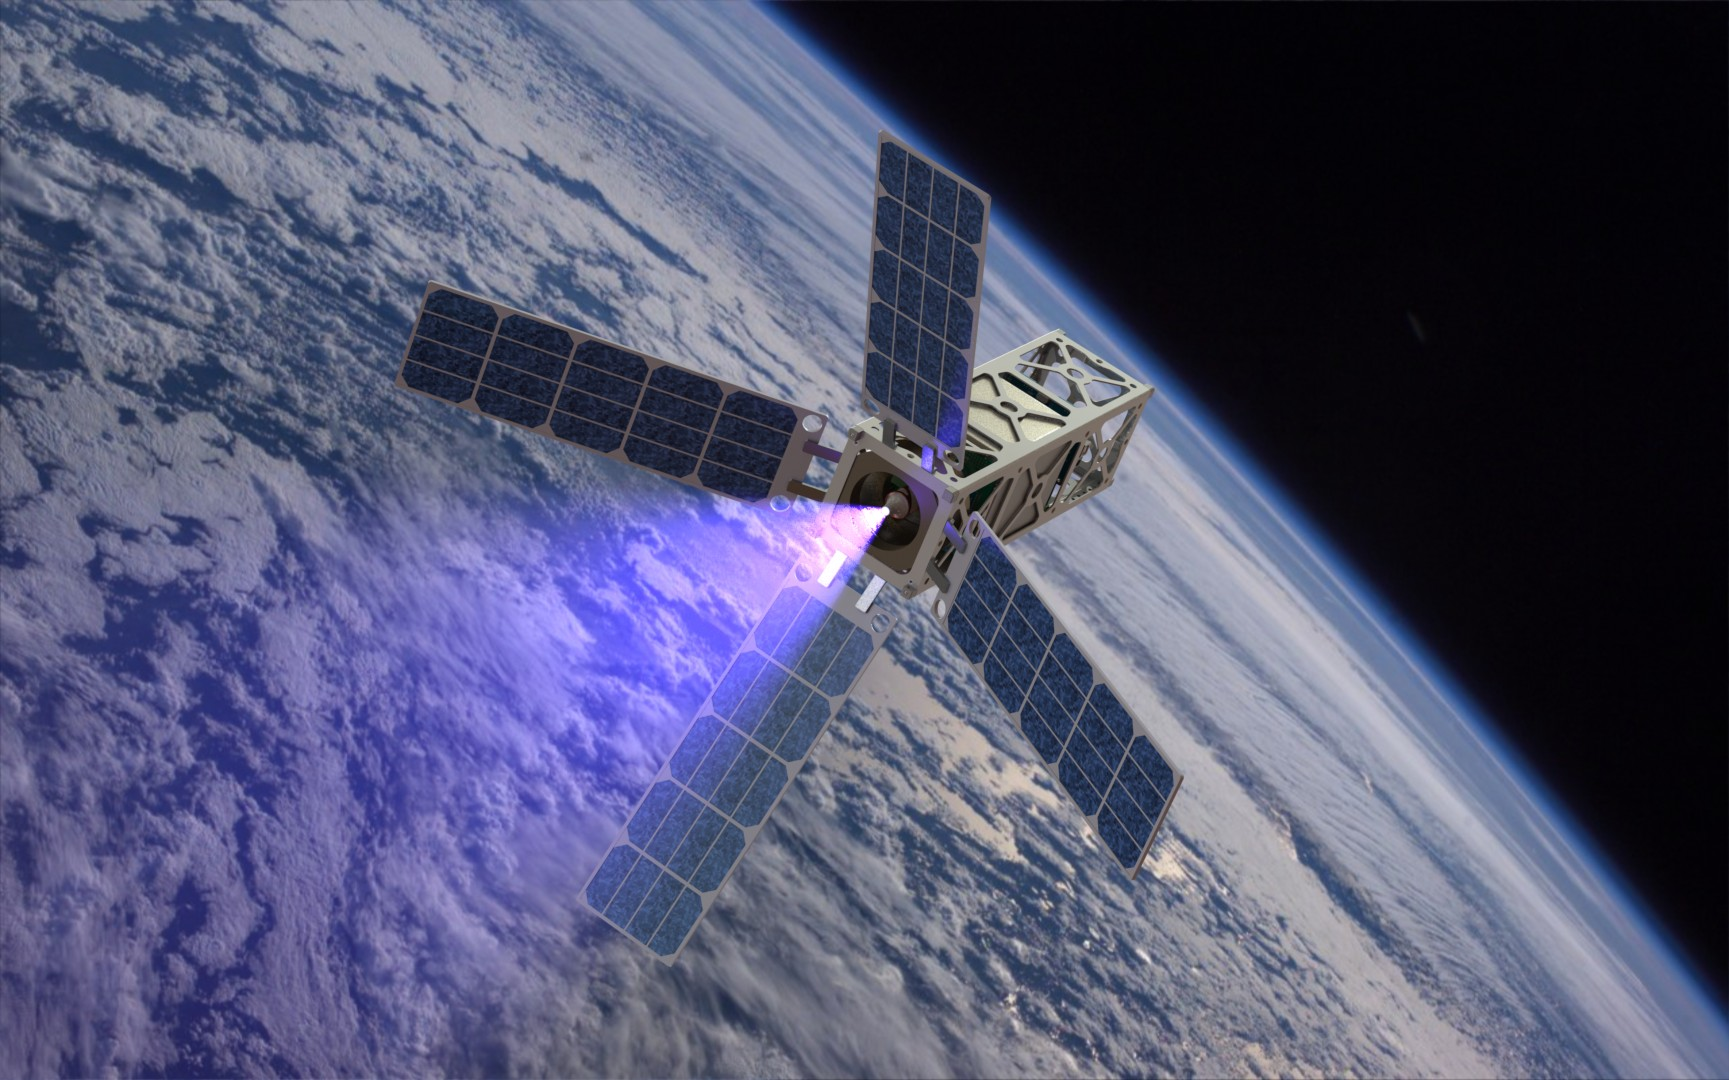
\includegraphics[height=0.3\textheight]{figures/2016AAS/patriot_plume.jpg}
        \hfill
        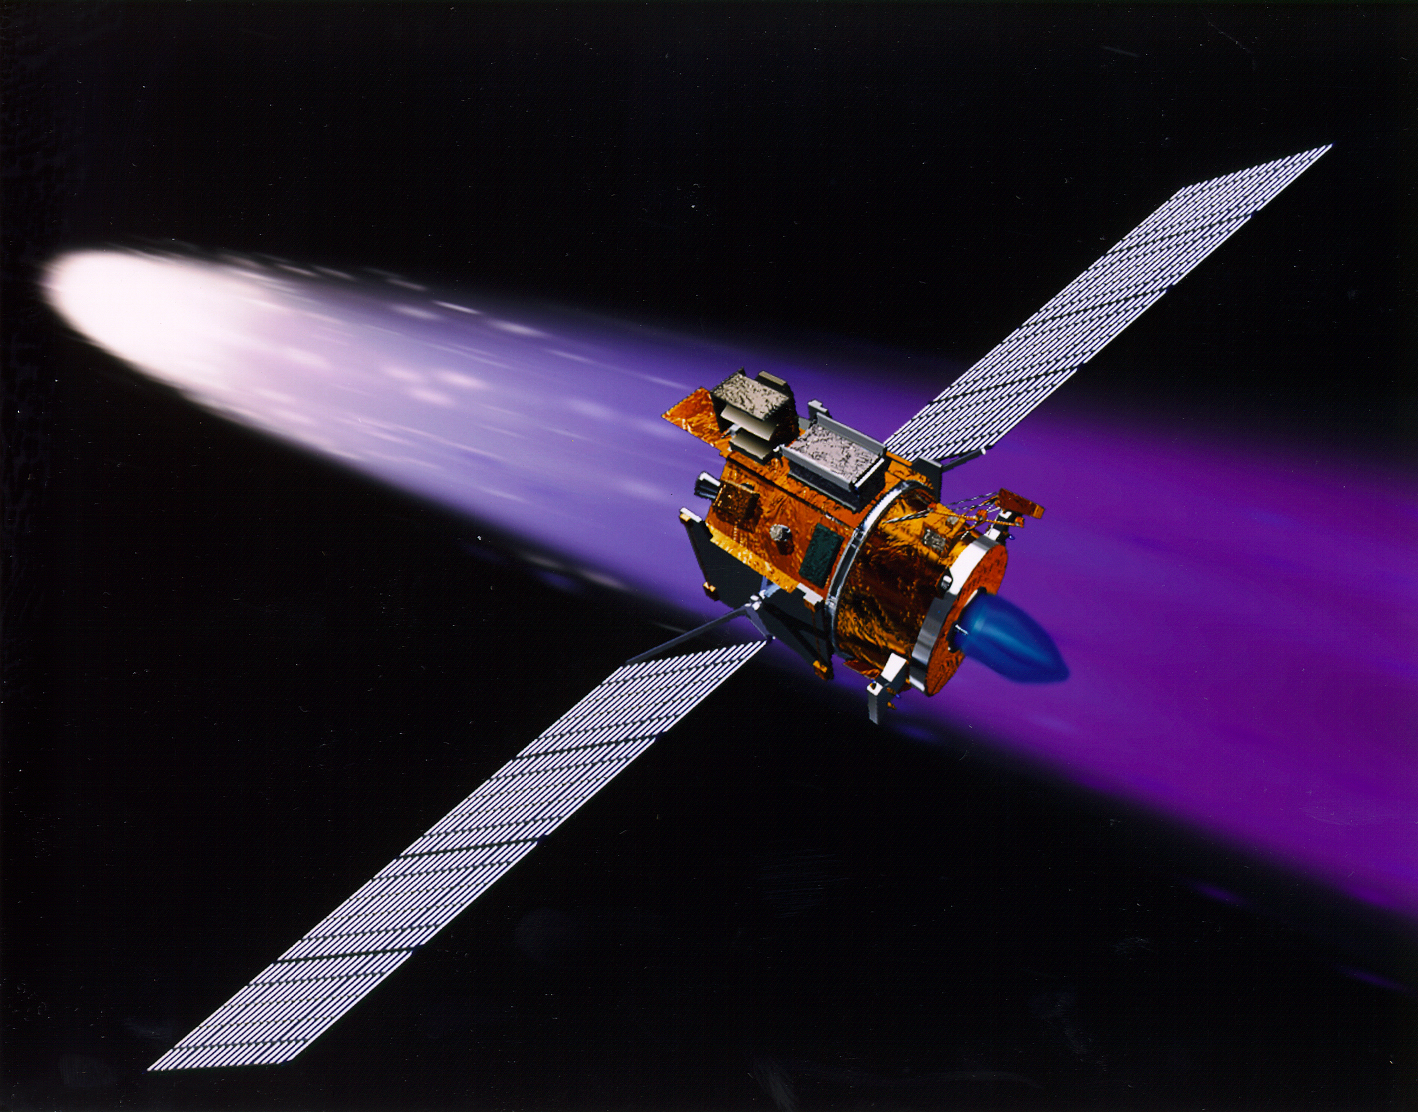
\includegraphics[height=0.3\textheight]{figures/2016AAS/deepspace1.jpg}
 
        \item Offers much higher specific impulse than chemical engines 
        
        \item Requires much longer operating periods for maneuvers 
        \item Small satellites with electric propulsion allows for new mission types
            \begin{itemize}
                \item Formation flight (distributed aperture sensing)
                \item On-orbit servicing
                \item Interplanetary swarms
            \end{itemize}
    \end{itemize}
\end{itemize}
\end{frame}   %-----------------------------%

\begin{frame} %-----------------------------%
\frametitle{Low-thrust vehicles} % electric propulsion
\begin{itemize}
    \item Low-thrust orbital transfers offer increased mission oportunities
    \begin{itemize}
        \item Electric propulsion is increasing in capability
        \item Offers much higher specific impulse than chemical engines 
        \item Requires much longer operating periods for maneuvers 
        \item Enables long duration missions with frequent thrusting
    \end{itemize}
\end{itemize}

\begin{center}
    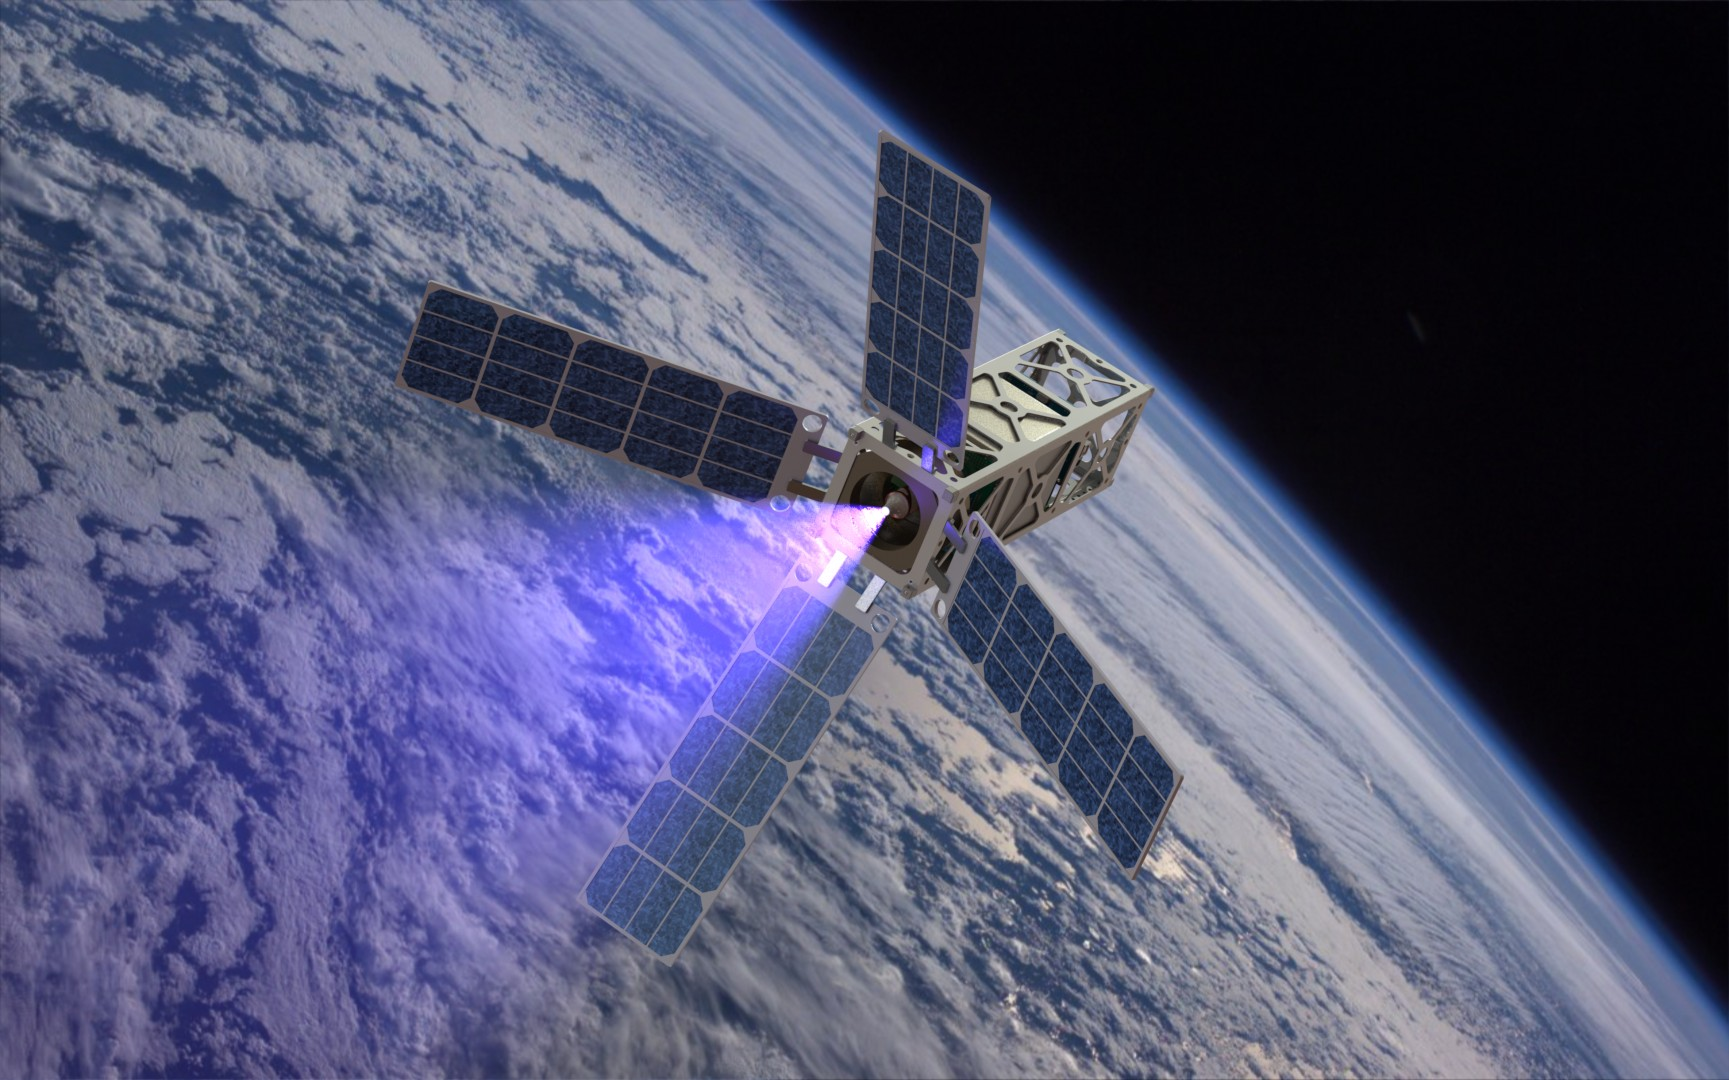
\includegraphics[width=0.5\textwidth,height=0.5\textheight,keepaspectratio]{figures/2016AAS/patriot_plume.jpg}
    ~
    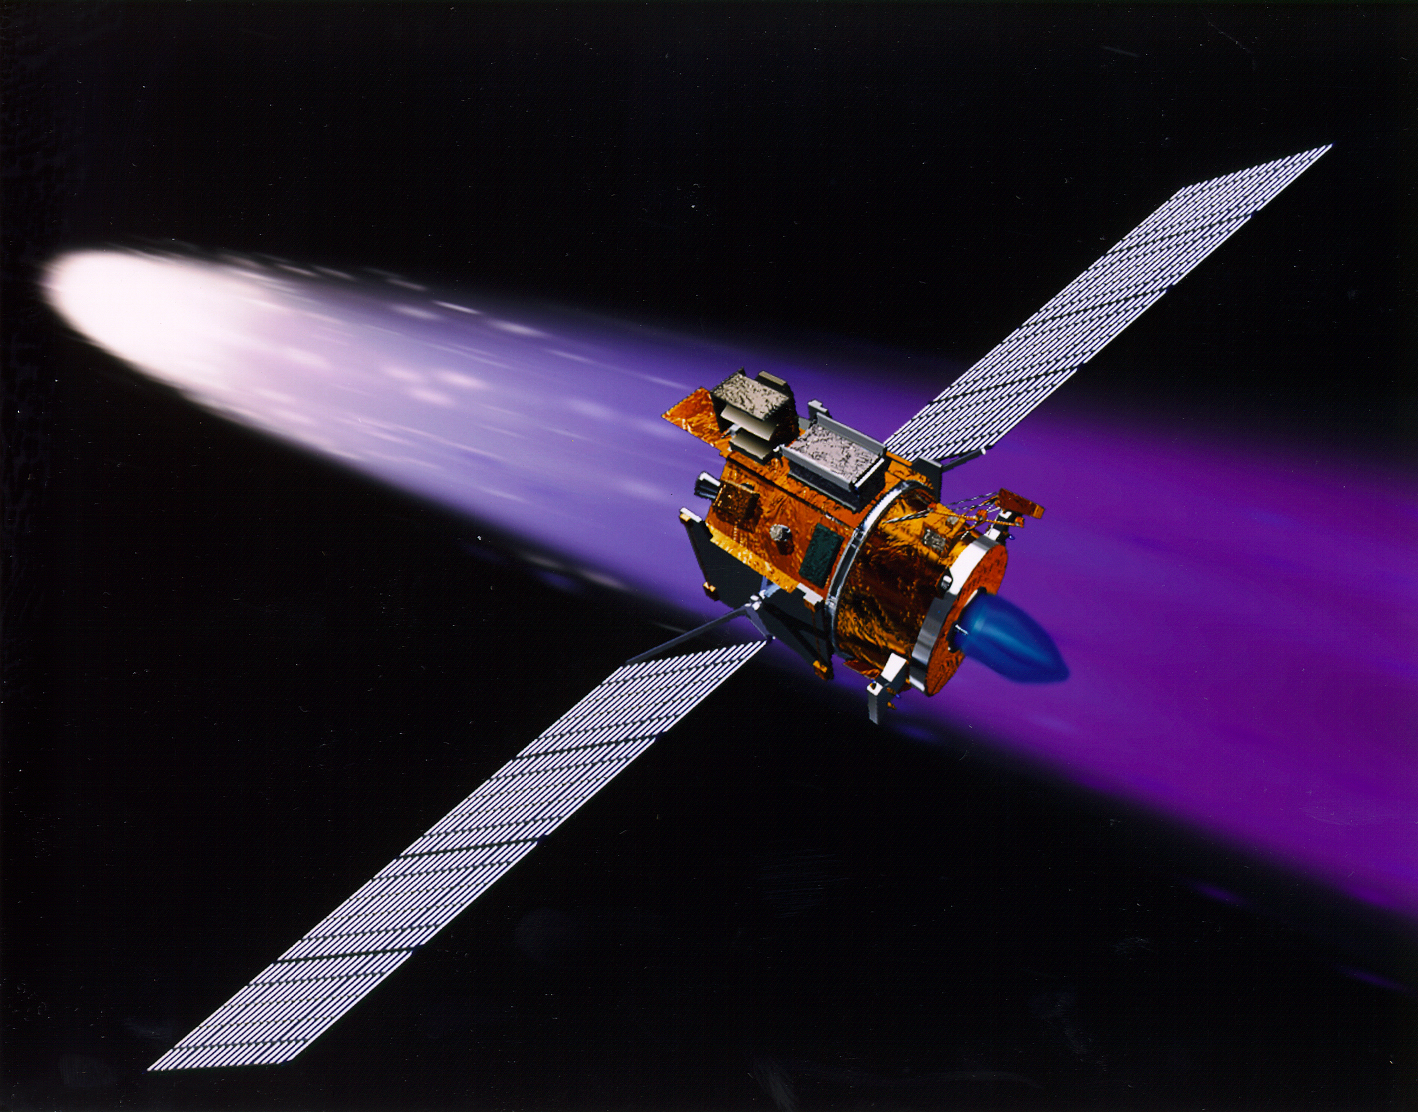
\includegraphics[width=0.5\textwidth,height=0.5\textheight,keepaspectratio]{figures/2016AAS/deepspace1.jpg}
\end{center}
\end{frame}   %-----------------------------%

